%%%%%%%%%%%%%%%%%%%%%%%%%%%%%%%%% Hauptteil %%%%%%%%%%%%%%%%%%%%%%%%%%%%%%%%%%

\chapter{Hauptteil}
\label{chap:Hauptteil}

\section{Grundlegende Überlegungen zur Durchführung des Projektes}
Das Projektseminar „Erstellung eines Zeitplan-Generators für Leichtathletikveranstaltungen“ wird von Thomas Baumer und Benedikt Bruckner (beide 5. Semester Wirtschaftsinformatik) unter Betreuung von Gerit Wagner durchgeführt. Als erstes stellte sich die Frage wie das Projekt umgesetzt werden soll und welche Software bzw. Programmiersprache zur Problemlösung verwendet werden sollen. 
Für die Wahl einer Programmiersprache zwischen JavaScript und Python konnte schnell eine Entscheidung getroffen werden, obwohl JavaScript und Python beides Sprachen sind für die eine Vielzahl an Dokumentationen, Bibliotheken und Tutorials existieren. Zudem wird ein klares und übersichtliches Programmieren bei beiden ermöglicht. Da Thomas Baumer und Benedikt Bruckner aber bereits im Kurs „Internettechnologien und Network-Computing“ erste Erfahrungen in JavaScript sammeln konnten, entschied man sich für JavaScript und sparte sich so eine größere Einarbeitungszeit in eine neue Programmiersprache. Mit der Verwendung von JavaScript können alle gewünschten Ziele erreicht werden.
Des Weiteren wurde die Verwendung einer Versionsverwaltungssoftware diskutiert. Da eine Versionsverwaltung viele Vorteile bietet, wie beispielsweise das Wiederherstellen von alten Zuständen des Projekts und die Protokollierung, wo jede Änderung an den Dateien mit Autor und Datum, also die ganze Versionsgeschichte, nachvollzogen werden kann, entschied man sich auch schnell und eindeutig für die Möglichkeit einer Versionsverwaltung. Außerdem ist es viel leichter, nachvollziehbarer und übersichtlicher als beispielsweise das Verschicken von einzelnen Codeteilen per E-Mail an die anderen Projektteilnehmer. (Quelle: PdP-Skript) Zudem bietet eine Versionsverwaltung noch die Möglichkeit Zugriffe und Entwicklungszweige zu koordinieren, was jedoch bei diesem Projekt aufgrund der Komplexität hinsichtlich der Projektteilnehmer nicht zwingend notwendig ist. Als Versionsverwaltungssoftware einigte man sich schließlich auf den „GitHub Desktop“, da man schon im Kurs „Praxis des Programmierens“ positive Erfahrungen mit Git sammeln konnte. 
Als Editor zur Erstellung von html- bzw. JavaScript-Code wurde einerseits unter Windows Notepad++ und andererseits für Mac die Software Brackets verwendet, da diese Open Source-Editoren sind und viele Sprachen, wie beispielsweise JavaScript, jQuery und html unterstützen. Sie genügen also allen im Projekt erwartenden Ansprüchen.
Bei der Entwicklung wurde vordergründig der Browser Google Chrome verwendet, da dieser alle verwendeten Sprachen, Frameworks und Methoden unterstützt. 
Ein weiteres Ziel ist eine fertige Desktop-App zu entwickeln. Dafür macht man sich die Software node.js zunutze. Der Vorteil hier ist, dass nach dem Erstellen des eigentlichen Programms mit dem Editor nur noch kleine Anpassungen vorgenommen werden müssen, um ein fertiges Programm zu erhalten. Dies hat die positive Auswirkung, dass der Nutzer nicht extra die verschiedenen html-Dateien abspeichern muss, womit er sich möglicherweise auch nicht sehr gut auskennt. Ein eigenständiges Programm erleichtert die Bedienbarkeit und die Nutzerfreundlichkeit. 
Darüber hinaus diskutierte man zu diesem frühen Stadium des Projektes bereits wie die abschließende Projektseminararbeit geschrieben werden soll. Betreuer Gerit Wagner empfahl die Verwendung des Softwarepaketes LaTex, das bei der Erstellung von größeren Abschlussarbeiten viele Vorteile gegenüber Microsoft Office Word bietet, abgesehen von dem Nachteil der Einarbeitungszeit in die ungewohnte Umgebung. Ein Argument ist, dass LaTex die Formatierung und den Inhalt voneinander trennt, indem man zu verändernde Textstellen mit Befehlen in einem Editor kennzeichnet, was ein sauberes und genau festlegbares Layout zur Folge hat. (https://de.wikipedia.org/wiki/LaTeX ) Außerdem gibt es seitens des Lehrstuhls bereits eine LaTex-Vorlage für Projektseminararbeiten auf die zurückgegriffen werden kann. Somit können die strengen Anforderungen für die Formatierung bzw. Gestaltung einer umfangreichen Projektseminarabschlussarbeit durch ein sauberes Layout erzielt werden. Zudem gibt es bereits grafische Editoren die den Umgang mit LaTex vereinfachen. Im Rahmen des Projekts wurde die Software TeXworks verwendet. Des Weiteren kann man für LaTex-Dokumente wieder ein Git-Repository anlegen und so alle Vorteile einer Versionsverwaltung nutzen.

\section{Beispiele}
Dies  ist eine Referenz auf ein Paper \cite{Kolter2009}. Die Verwaltung der Referenzen erfolgt in der Datei References.bib. Zur Bearbeitung der Referenzen kann beispielsweise das Programm JabRef\protect{\footnote{\url{http://jabref.sourceforge.net/}}} verwendet werden.

Besonders interessant ist auch die automatische Erstellung des Abkürzungsverzeichnisses. Zuerst wird die Abkürzung definiert um bei erstmaliger Verwendung im Abkürzungsverzeichnis zu erscheinen: \ac{Bsp.}, \ac{SaaS}

Referenzen auf Grafiken: \ref{fig:Fig1}, \ref{img:subFig2}, \ref{img:subFigs}

\begin{figure}
  \centering
  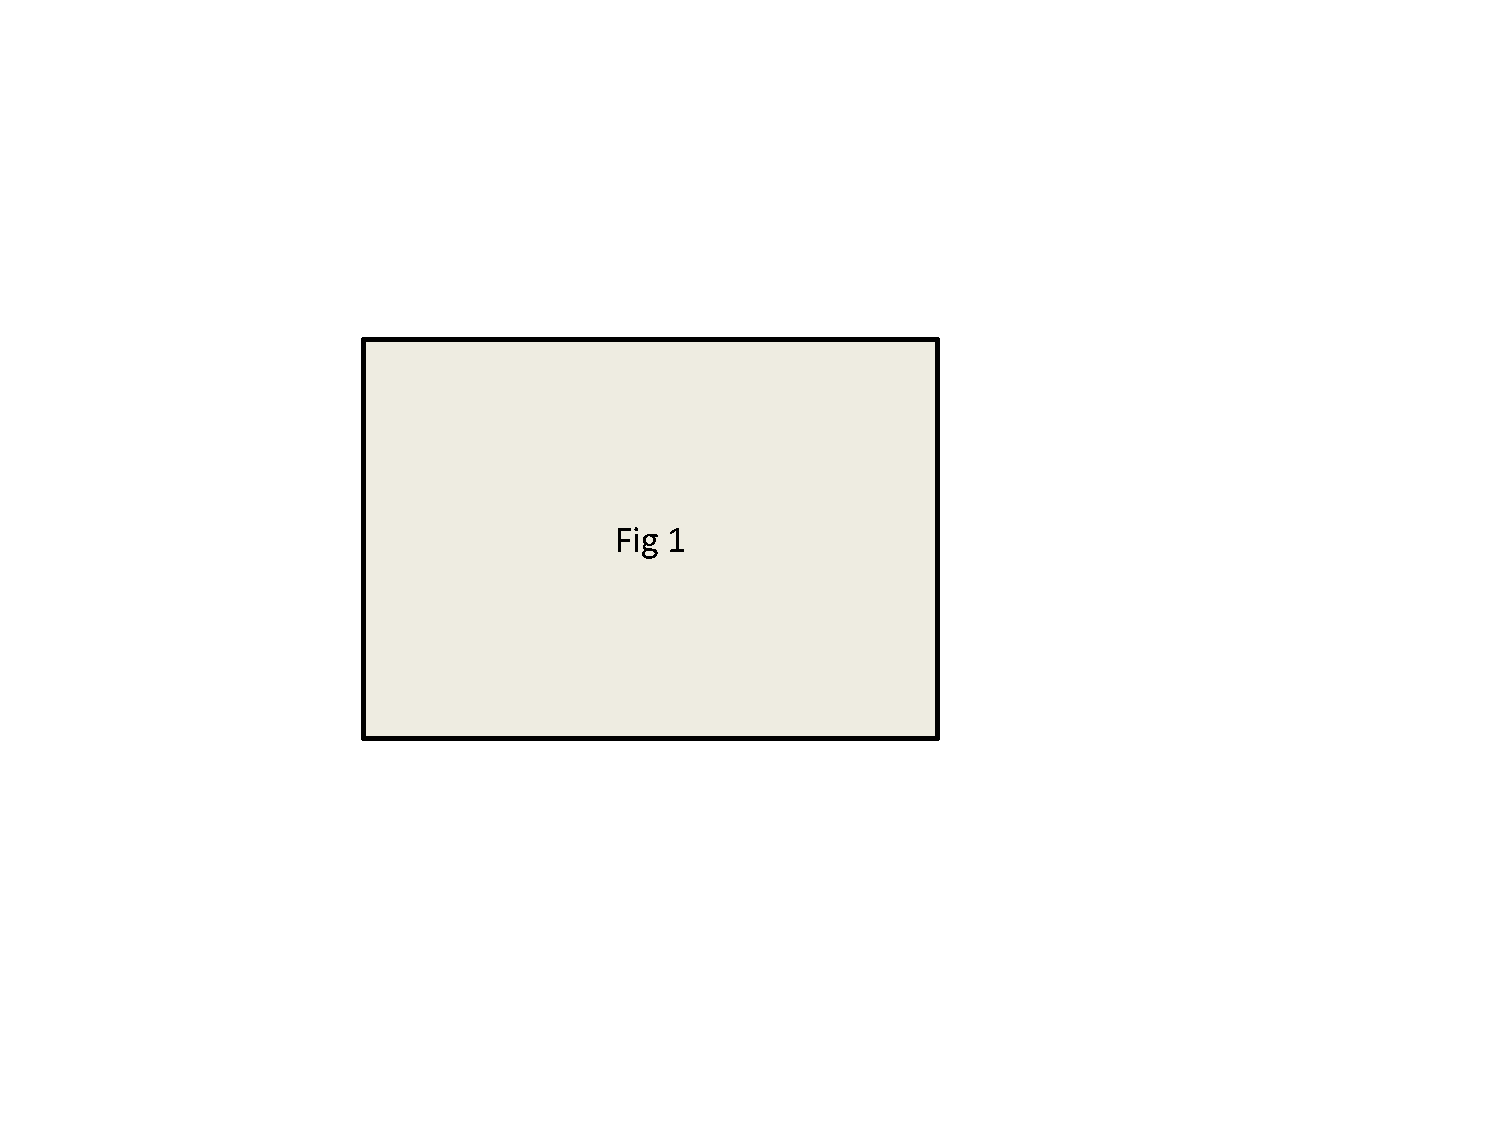
\includegraphics[width=0.95\textwidth]{Fig1.pdf}
  \caption{Beispielgrafik}
  \label{fig:Fig1}
\end{figure}


\begin{figure}
  \centering
  \subfigure[subfigure 1 \label{img:subFig1}]{\fbox{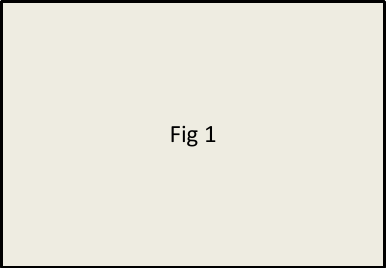
\includegraphics[width=0.45\textwidth]{Fig.png}}}\hfill
  \subfigure[subfigure 2\label{img:subFig2}]{\fbox{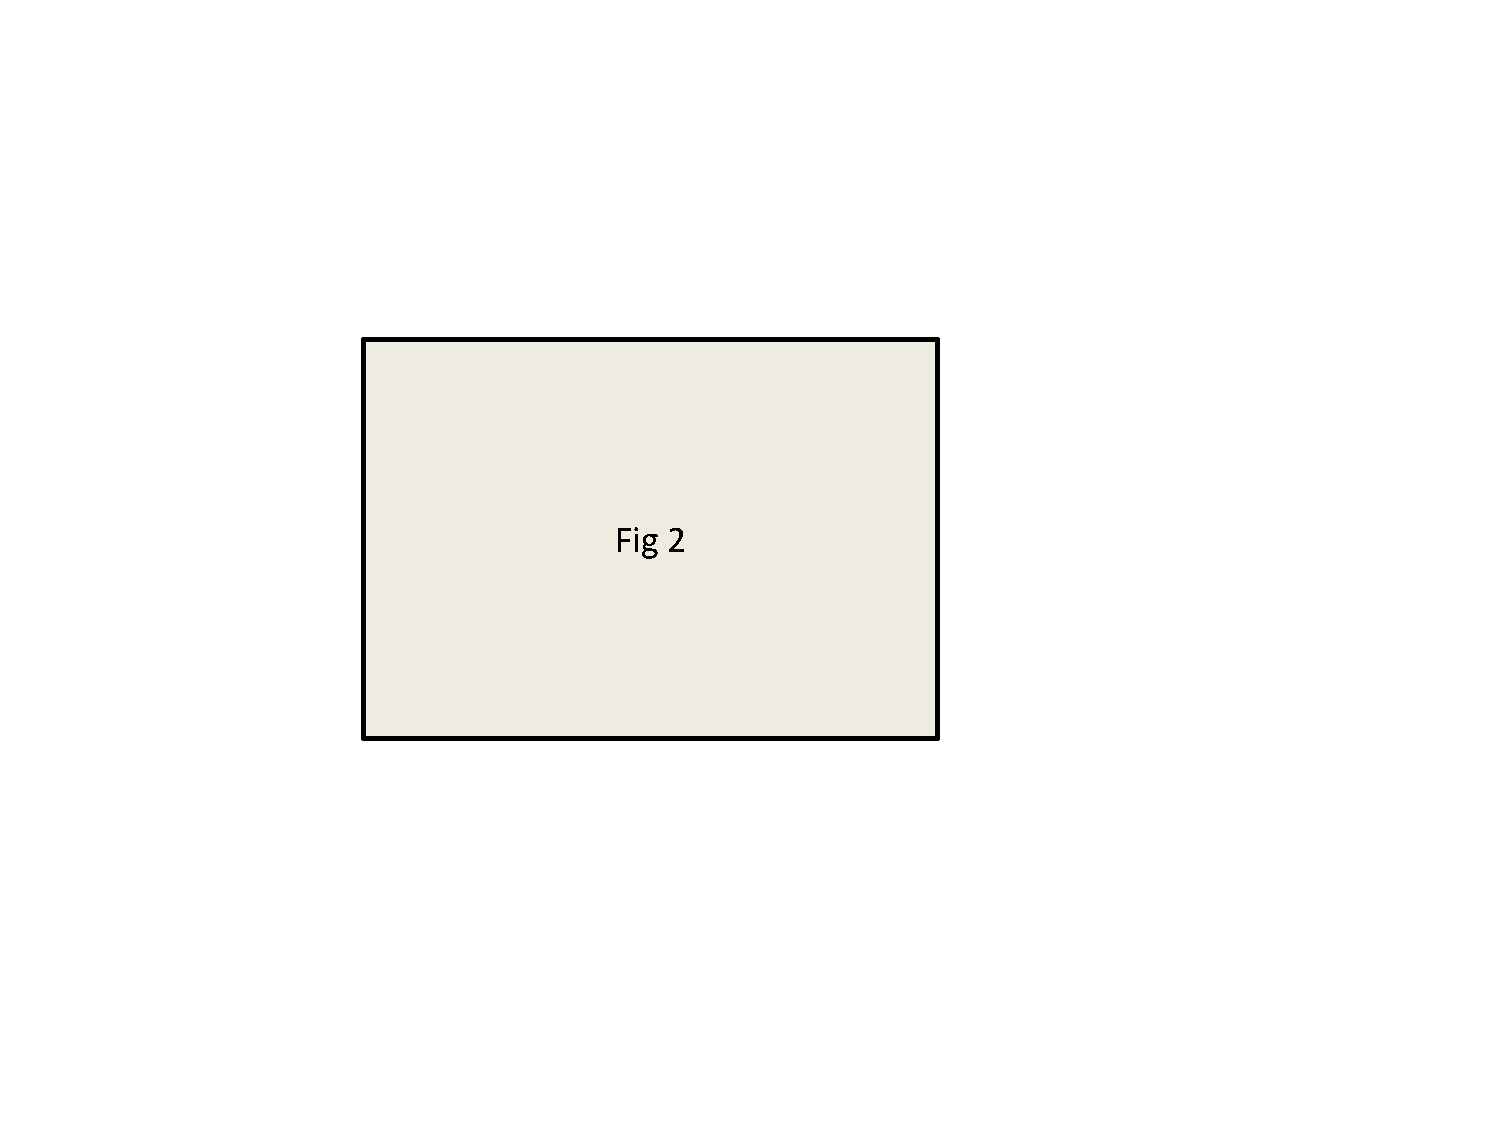
\includegraphics[width=0.45\textwidth]{Fig2.pdf}}}\hfill
  \caption{Beispiel subfigure}
  \label{img:subFigs}
\end{figure}



\lstset{language=JAVA, breaklines=true, tabsize=2}
\lstinputlisting[caption=HelloWorld,
label=lst:HelloWorld]{listings/HelloWorld.java}


%%%%%%%%%%%%%%%%%%%%%%%%%%%%%%%%%%%%%%%%%%%%%%%%%%%%%%%%%%%%%%%%%%%%%%%%%%%%%%
